% ****** Start of file apssamp.tex ******
%
%   This file is part of the APS files in the REVTeX 4.2 distribution.
%   Version 4.2a of REVTeX, December 2014
%
%   Copyright (c) 2014 The American Physical Society.
%
%   See the REVTeX 4 README file for restrictions and more information.
%
% TeX'ing this file requires that you have AMS-LaTeX 2.0 installed
% as well as the rest of the prerequisites for REVTeX 4.2
%
% See the REVTeX 4 README file
% It also requires running BibTeX. The commands are as follows:
%
%  1)  latex apssamp.tex
%  2)  bibtex apssamp
%  3)  latex apssamp.tex
%  4)  latex apssamp.tex
%
\documentclass[%
%  reprint,
%superscriptaddress,
%groupedaddress,
%unsortedaddress,
%runinaddress,
%frontmatterverbose,
%preprint,
%preprintnumbers,
%nofootinbib,
%nobibnotes,
%bibnotes,
 amsmath,amssymb,
%  aps,
%pra,
%prb,
%rmp,
%prstab,
%prstper,
%floatfix,
]{revtex4-2}

\usepackage{graphicx}% Include figure files
\usepackage[caption = false]{subfig}
% \usepackage{dcolumn}% Align table columns on decimal point
\usepackage{bm}% bold math
\usepackage{soul}
\usepackage{todonotes}
\usepackage{mathtools}

%New command that lets you draw double overlines easily. Just use $ \Overline{variable}$
\newcommand{\Overline}[1]{\overline{\overline{#1}}}
\newcommand{\rmd}[0]{\mathrm{d}}
\setlength{\parskip}{3.5mm}

\DeclarePairedDelimiter\abs{\lvert}{\rvert}
\makeatletter
\let\oldabs\abs
\def\abs{\@ifstar{\oldabs}{\oldabs*}}
%\usepackage{hyperref}% add hypertext capabilities
%\usepackage[mathlines]{lineno}% Enable numbering of text and display math
%\linenumbers\relax % Commence numbering lines

%\usepackage[showframe,%Uncomment any one of the following lines to test
%%scale=0.7, marginratio={1:1, 2:3}, ignoreall,% default settings
%%text={7in,10in},centering,
%%margin=1.5in,
%%total={6.5in,8.75in}, top=1.2in, left=0.9in, includefoot,
%%height=10in,a5paper,hmargin={3cm,0.8in},
%]{geometry}

\begin{document}


\title{Entropy Production in a Current-Free System}% Force line breaks with \\

\author{Jacob Knight}

\author{Farid Kaveh}

\author{Gunnar Pruessner}%


\affiliation{%
 Imperial College London
}%

\begin{abstract}

We derive the leading-order contribution to the entropy production of two current-free systems in closed form. Both systems are derived from a one-dimensional Run-and-Tumble (RnT) particle with a hidden degree of freedom. These are the first examples of a closed-form expression for the entropy production rate of non-Markov systems. We furthermore develop a perturbation theory to systematically calculate the entropy production rates of processes operating in continuous space and time with hidden degrees of freedom. In particular, our method enables the calculation of the entropy production rate of irreversible processes with no net current.
% We develop a perturbation theory to systematically calculate the entropy production rates of processes operating in continuous space and time with hidden degrees of freedom. Our methods go beyond previously proposed procedures for systems moving between finitely-many states. In particular, our method enables the calculation of the entropy production rate of irreversible processes with no net current. This is demonstrated for two paradigmatic examples: an asymmetric Run-and-tumble (RnT) particle in free space and a symmetric RnT particle in a harmonic potential.
\end{abstract}

%\keywords{Suggested keywords}%Use showkeys class option if keyword
                              %display desired
\maketitle

\section{Introduction}
A pressing open question in the field of active matter concerns the possibility of extracting useful work from self-propelled particles, which include bacteria such as \textit{E. Coli} or synthetic colloids. The key quantity of relevance in determining the maximum possible power which can be extracted from a system is the entropy production rate \textit{(Good reference for this??)}. Significant efforts have already been made to calculate the entropy production rates of a wide range of models of physical systems \textit{Bunch of references here}. In all works referenced here, it is assumed that observers have complete access to all dynamical degrees of freedom in their models, which renders the systems Markovian.

Real systems are more complicated. Observers usually lack information about some hidden set of degrees of freedom, which may vary stochastically at inaccessibly short time and length scales. Upon removal of an observer's access to a subset of the total degrees of freedom, the behaviour of the remaining degrees of freedom becomes non-Markov, despite the fact that the underlying dynamics remain unchanged. Previous formulations of the entropy production rate have been unable to deal with



Stochastic thermodynamics provides a framework for extending extensive thermodynamic quantities such as work, heat, and energy to  microscopic and mesoscopic systems. Such systems are commonly found in the context of active matter, as well as in biological tissue modelling and quantum mechanics. The entropy production of such systems has been the subject of particular interest. The entropy production distinguishes systems on their path to equilibrium, and those with fluctuations around the equilibrium state, from ensembles that exhibit true Non-Equilibrium Steady States (NESS).  \todo{reference} This characterisation is cruicial to understanding the nature of energy dissipation in any system. For systems far-from-equilibrium, the entropy production governs the rate of approach to equilibrium through the relevant fluctuation theorem.\todo{reference} Moreover, the entropy production bounds the free energy cost of maintaining a process, see for example \cite{SONG2019R566,RODENFELS2019646} for discussions on the relationship between heat flow and the energy cost of embryonic processes.

For systems driven by Markovian dynamics the rate of entropy production can be deduced from the master equation (discrete state-space)\todo{ref Schnakenberg} or the Langevin equation (continuous state-space).\todo{reference} Examples of Markovian systems whose entropy productions can be exactly solved can be found in the context of molecular engines, chemical reactions, and quantum systems \cite{Bio-uncertainty-relation}\todo{ref Luca}.  While many different schemes for the entropy production of non-Markovian systems have been studied, a survey of the literature reveals no reference models.

Here we derive a perturbative expression for the entropy production of a diffusion process whose self-propulsion rate is governed by a hidden stochastic process independent of the noise.  This hidden degree of freedom renders the process non-Markov.  We apply this result to obtain the first-order contribution to the entropy production when the hidden process is an asymmetric telegraph process. We also extend to the case where the diffusion process is confined in a harmonic potential. To the authors' knowledge, this is the first example of a closed form expression for the entropy production of a non-Markovian process.

%  An important feature of many non-equilibrium models is the appearance of Non-Equilibrium Steady States (NESS).\todo{find reference} These are statistical steady states where the system is not in thermal equilibrium. This may occur for example as a result of a particular arrangement of heat reservoirs that makes it impossible for the system to achieve equilibrium,\cite{schnakenberg1976network} or, as is the case in many biological settings, it may result from the conversion of free energy into motion at a microscopic level.\cite{Mechs-Stats-Active, nardini2017entropy}

% A key statistical property of a non-equilibrium system is its time averaged entropy production.
% For the case of NESS for finite, closed Markov processes, Schnakenberg provides a general expression for the entropy production in the steady state,\cite{schnakenberg1976network}. Recent research focuses on non-Markov systems whose statistics remain largely unresolved.\cite{kutvonen2015entropy,loos2019heat,garcia2012nonadiabatic}
\ldots end intro \ldots

A case of particular interest is when $w(t)$ follows a telegraph process (FIND CITATION), switching between two values $w_1$ and $w_2$ with with Poissonian rates $\alpha_1$ and $\alpha_2$ respectively (INSERT FIGURES HERE - two state process with arrows and rates, and typical w trajectory).

We consider the situation where an observer of this process only has knowledge of the trajectory of the particle in position space, denoted $\{\dot{x}(t)\}$, and not of the telegraph process $w(t)$. Given this incomplete description the process is no longer Markov. This is because, letting $\tau$ be a time increment such that $\alpha_1\tau, \alpha_2\tau << 1$, the net movement of the particle in time $\tau$ is strongly correlated with the instantaneous state of the hidden variable $w(t)$.
The probability of the path $\{\dot{x}(t)\}$ having occurred is denoted by $\mathcal{P}\left[\{\dot{x}(t)\}\right]$. When the trajectory of the self propulsion velocity $\{w(t)\}$ is also known to the observer, the subsequent evolution of ....

The observable of interest is the entropy production rate, which measures the distance of a process from equilibrium. It is given by (REFERENCE GASPARD)

\begin{equation}\label{EP}
    \dot{\mathcal{S}} = \lim_{T \to \infty} \frac{1}{T}  \left\langle \ln\left(\frac{\mathcal{P}[\{\dot{x}\}]}{\mathcal{P}[\{\dot{x}\}^R]}\right) \right\rangle
\end{equation}


\section{Derivation of entropy production rate}\label{methods}

Consider a self-propelling particle whose motion is described by the Langevin equation
\begin{equation}\label{langevin}
\begin{split}
        \dot{x}(t)&= \nu w(t)- \frac{\partial V}{\partial x} +\xi(t)\\
        \langle \xi(t) \xi(t') \rangle &= 2 D \delta(t-t')
\end{split}
\end{equation}
where $x(t)$ and $w(t)$ are the position and self-propulsion velocity of the particle respectively, $\nu$ is a dimensionless bookkeeping parameter, $V = V(x)$ is a potential expressed in units of velocity, and $\xi(t)$ represents white noise with diffusion constant D.

We seek to express the probability of a specific realisation of a velocity trajectory $\{\dot{x}(t)\}$ occurring as a result of the dynamics (\ref{langevin}). It is first assumed that the trajectory of the self-propulsion $\{w(t)\}$ is known. Using the fact that the noise $\xi(t)$ follows a Gaussian distribution (Onsager-Machslup(ref?))
\begin{equation}\label{fulldist}
    \mathcal{P}\left[\{\dot{x}(t)\}|\{w(t)\}\right] \propto \exp \left\{-\frac{1}{4D} \int \rmd t \left(\dot{x} + \frac{\partial V}{\partial x}-\nu w\right)^2
    \right\}
\end{equation}
By marginalising over all possible trajectories $\{w(t)\}$, we arrive at the probability of the realisation of a spatial path $\{\dot{x}(t)\}$, $\mathcal{P}\left[\{\dot{x}(t)\}\right]$\st{which makes no reference to a trajectory of the self-propulsion velocity $w(t)$}. Introducing the following notation for clarity:
\begin{equation}\label{doubleoverline}
\begin{split}
        \Overline{\bullet}&=\int \mathcal{D}{w(t)}\mathcal{P}\left[\{w(t)\}\right]\bullet \\
\end{split}
\end{equation}
the spatial path probability may be expressed from equation (\ref{fulldist}) as

\begin{equation}
\begin{split}
\mathcal{P}\left[\{\dot{x}(t)\}\right] &= \Overline{\mathcal{P}\left[\{\dot{x}(t)\}|\{w(t)\}\right] } \\
&= \exp \left(-\frac{1}{4D} \int \rmd t \left(\dot{x}+ V'\right)^2 \right) \Overline{\exp \left(-\frac{1}{4D} \int \rmd t (-2\dot{x}\nu w- 2\nu w V' + (\nu w)^2)\right)}
\end{split}
\end{equation}
% Using equation (\ref{fulldist}) we can write the path probability marginalised over ${w(t)}$:
% \begin{equation}\small
%             \mathcal{P}\left[\{\dot{x}(t)\}\right] = \exp \left(-\frac{1}{4D} \int \rmd t \dot{x}^2 \right) \Overline{\exp \left(-\frac{1}{4D} \int \rmd t (-2\dot{x}\nu w + (\nu w)^2)\right)}
% \end{equation}

\subsection{Perturbation Theory}

We proceed by expanding perturbatively in the dimensionless velocity coefficient $\nu$:
\begin{equation}\small
\begin{split}
     \mathcal{P}\left[\{\dot{x}(t)\}\right] = &\exp \left(-\frac{1}{4D} \int \rmd t \left(\dot{x}+V' \right)^2 \right) \bigg[1+\frac{\nu}{2D}\int \rmd t \Overline{w(t)}\left( \dot{x}(t) + V'\right) \\ &+ \nu^2 \left(-\frac{1}{4D}\int \rmd t \Overline{w^2(t)} + \frac{1}{8D^2}\int \rmd t_1 \rmd t_2 \Overline{w(t_1)w(t_2)}\left(\dot{x}(t_1)\dot{x}(t_2) + 2\dot{x}(t_1)V' + (V')^2\right)\right) \\
     &+ \nu^3 \left( -\frac{1}{8D^2}\int \rmd t_1\rmd t_2 \Overline{w^2(t_1)w(t_2)}(\dot{x}(t_1) + V') + \frac{1}{48D^3}\int \rmd t_1 \rmd t_2 \rmd t_3 \Overline{w(t_1)w(t_2)w(t_3)}\prod_{i=1}^3(\dot{x}(t_i)+V') \right) + \mathcal{O}(\nu^4) \bigg]
\end{split}
\end{equation}

This allows us to express the average entropy production rate of a \textit{specific trajectory} $\{\dot{x}(t)\}$ of duration $T$ (REFERENCE):

\begin{widetext}
\begin{equation}\small\label{onepath}
\begin{split}
 \dot{\mathcal{S}}(\{\dot{x}(t)\}) = & \frac{1}{T}\ln\left(\frac{\mathcal{P}\left[\{\dot{x}(t)\}\right]}{\mathcal{P}\left[\{\dot{x}(t)\}^R\right]}\right) \\= &  - \frac{1}{TD}\int^T_0 \dot{x}(t)V' \rmd t+ \frac{\nu}{TD}\int_0^T\rmd t\dot{x}(t)\Overline{w(t)} \\
 &- \frac{\nu^2}{T}\frac{1}{2D^2}\int^T_0 \rmd t_1 \rmd t_2 \Overline{w(t_1)w(t_2)}\dot{x}(t_1)V' \\
 &+ \frac{\nu^3}{T} \bigg[\frac{1}{4D^2} \int_0^T \rmd t_1 \rmd t_2 \Overline{w(t_1)}\cdot\Overline{w(t_2)^2}\dot{x}(t_1) + \frac{1}{24D^3}\int_0^T \rmd t_1 \rmd t_2 \rmd t_3 \Overline{w(t_1)w(t_2)w(t_3)}\left(\dot{x}(t_1)\dot{x}(t_2)\dot{x}(t_3) + 3\dot{x}(t_1)(V')^2\right)\\
  &- \frac{1}{8D^3}\int_0^T \Overline{w(t_1)}\cdot \Overline{w(t_2)w(t_3)}\left(\dot{x}(t_1)\dot{x}(t_2)\dot{x}(t_3)+ 3 \dot{x}(t_1)(V')^2\right)\bigg] + \mathcal{O}(\nu^4)
\end{split}
\end{equation}
\end{widetext}


The average entropy production rate $\dot{\mathcal{S}}$ of the process (\ref{EP}) is obtained by taking the expectation value of (\ref{onepath}) over $\dot{x}(t)$ and taking the limit as $T \rightarrow \infty$.

\textbf{We expanded up to order $\nu^3$, but the contributions we find are smaller than this. We can do this because $w$, $x$, and $V$ never appear alone in any term, but they always accompany each other at least in pairs. This means that the contribution from terms that are $\mathcal{O}(\nu^4)$ is at most $\mathcal{O}(\nu^8)$.}

\section{Asymmetric Run-and-Tumble Process}
\label{run_and_tumble}

\subsection{Description of the process}

\begin{figure}[h]
\centering
\subfloat[Asymmetric telegraph process.\label{telegraph_diagram}]{%

\includegraphics[width = 0.5\textwidth]{tele-diagram-2.png}}
\hfill
\subfloat[A Sample path of.\label{sample_path}]{%
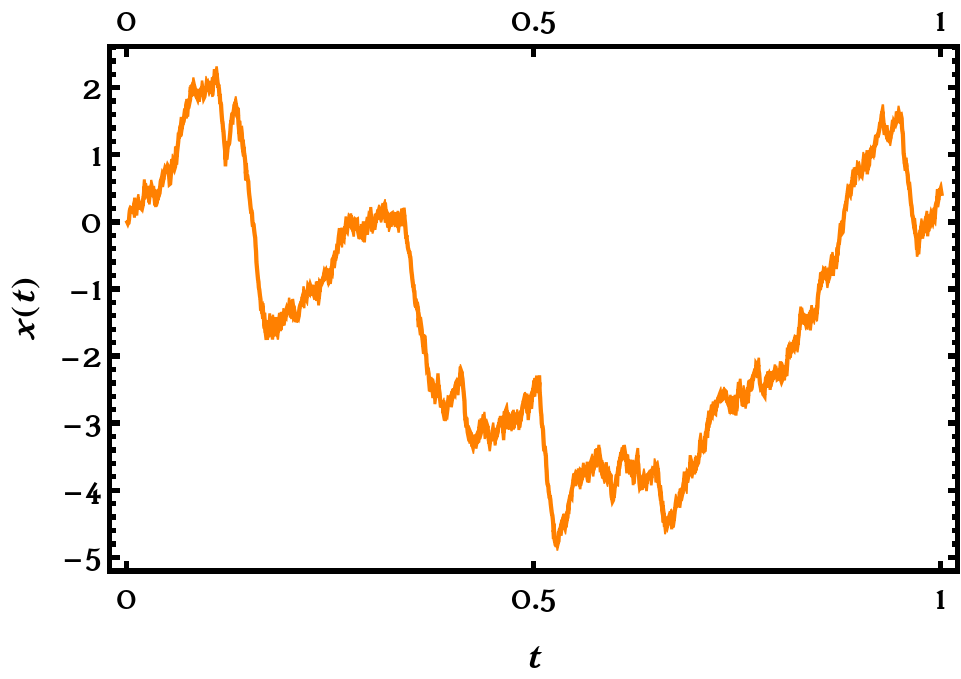
\includegraphics[width = 0.5\textwidth]{typica_tele_path_2.png}}
\caption{\ref{telegraph_diagram} shows a diagram of the telegraph process $w(t)$ as discussed in Section \ref{run_and_tumble}. In the +ve state, the particle has self-propulsion $\nu w_+$, and in the -ve state the self-propulsion is $\nu w_-$. Since $\Overline{w} = 0$, we have $\alpha_+w_- + \alpha_-w_+ = 0$. \ref{sample_path} depicts a sample path for the particle governed by \ref{langevin} where $w$ is an asymmetric telegraph process with zero mean.}
\label{figure1}
\end{figure}

We will now specialise to the case where $V \equiv 0$ and $w(t)$ is an asymmetric, mean-zero telegraph process. In other words, the Langevin equation now reads
\begin{equation}\label{free-run-tumble}
  \dot{x} = \nu w(t) + \xi(t),
\end{equation}

which describes an asymmetric RnT particle in one dimension. Note that in such a case we can easily deduce the n-th order autocorrelation function of $\dot{x}$ from Eqn. \ref{free-run-tumble}. We have

\begin{align}
    \langle \dot{x}\rangle &= \nu \Overline{w},\\
    \langle \dot{x}(t_1)\dot{x}(t_2) \rangle &= \nu^2 \Overline{w(t_1)w(t_2)} + 2D\delta(t_1-t_2), \\
    \langle \dot{x}(t_1)\dot{x}(t_2)\dot{x}(t_3) \rangle &= \nu^3 \Overline{w(t_1)w(t_2)w(t_3)},
\end{align}

Hence, by Eqn. (\ref{onepath}), the entropy production rate of such a process is

\begin{widetext}
\begin{equation}\label{RnT-entropy}\small
\begin{split}
 \dot{\mathcal{S}}= & \frac{\nu^2}{TD}\int_0^T\rmd t\left(\Overline{w(t)}\right)^2 +  \frac{\nu^4}{4TD^2} \int_0^T \rmd t_1 \rmd t_2 \left(\Overline{w(t_1)}\right)^2\cdot\Overline{w(t_2)^2} + \frac{\nu^6}{T} \bigg[\frac{1}{24D^3}\int_0^T \rmd t_1 \rmd t_2 \rmd t_3 \left(\Overline{w(t_1)w(t_2)w(t_3)}\right)^2\\
  &- \frac{1}{8D^3}\int_0^T \rmd t_1 \rmd t_2 \rmd t_3 \Overline{w(t_1)}\cdot \Overline{w(t_2)w(t_3)}\cdot\Overline{w(t_1)w(t_2)w(t_3)}\bigg] + \mathcal{O}(\nu^8)
\end{split}
\end{equation}
\end{widetext}



The telegraph process $w(t)$ switches between two values $w_+$ and $w_-$, with rates $\alpha_+$ and $\alpha_-$. These values are constrained by the zero-mean condition
\begin{equation}\label{zeromean}
    \Overline{w(t)} = \frac{w_+\alpha_- + w_-\alpha_+}{\alpha_+ + \alpha_-} = 0.
\end{equation}

Whenever this zero-mean condition is satisfied, the leading order contribution in Eqn. (\ref{RnT-entropy}) is given by

\begin{equation}\label{telEP}
\begin{split}
\boxed{
 \dot{\mathcal{S}}=  \frac{\nu^6}{24T D^3}\int_0^T\rmd t_1\rmd t_2\rmd t_3\left(\Overline{w(t_1)w(t_2)w(t_3)}\right)^2 }
\end{split}
\end{equation}


In the subsequent section, the three-time correlation function (and thus the leading-order entropy production) is derived in closed form.

\subsection{Calculation of three-time correlation function}
The asymmetric Run-and-Tumble process is represented by the master equation
\begin{equation}
\frac{d}{\rmd t}\begin{pmatrix}
p_+(t) \\
p_-(t)
\end{pmatrix} =
\begin{pmatrix}
-\alpha_+ & \alpha_- \\
\alpha_+  & -\alpha_-
\end{pmatrix}
\begin{pmatrix}
p_+(t) \\
p_-(t)
\end{pmatrix}
\end{equation}
where $p_+(t)$ is the probability of the process $w(t)$ taking the value $w_+$ at time $t$ and $p_-(t) = 1-p_+(t)$ is the probability that $w(t)$ takes the value $w_-$. This is solved exactly with appropriate boundary conditions and produces the following matrix elements:

\begin{equation}\label{elements}
    \begin{split}
        P_{++}(t) &= \frac{1}{\alpha_+ + \alpha_-} \left(\alpha_- + \alpha_+ e^{-(\alpha_+ + \alpha_-)t}\right) \\
        P_{-+}(t) &= \frac{1}{\alpha_+ + \alpha_-} \left(\alpha_+ - \alpha_+ e^{-(\alpha_+ + \alpha_-)t}\right) \\
        P_{+-}(t) &= \frac{1}{\alpha_+ + \alpha_-} \left(\alpha_- - \alpha_- e^{-(\alpha_+ + \alpha_-)t}\right) \\
        P_{--}(t) &= \frac{1}{\alpha_+ + \alpha_-} \left(\alpha_+ + \alpha_- e^{-(\alpha_+ + \alpha_-)t}\right) \\
    \end{split}
\end{equation}
where $P_{-+}(t)$ is the probability of $w(t)$ taking a value $w_-$ having been initialised at $t=0$ with value $w_+$. The three-time correlation function of $w(t)$ is expressed as follows:
\begin{equation}\label{3time}
\begin{split}
    \Overline{w(t_3)w(t_2)w(t_1)} =& \mathcal{I}(t_3>t_2>t_1)
 \begin{pmatrix}
1 & 1\\
\end{pmatrix}
M_{w}(t_3-t_{2})M_{w}(t_2-t_{1})
\begin{pmatrix}
w_+P_{+}\\
w_-P_{-}
\end{pmatrix}\\
&+\mathcal{I}(t_2>t_3>t_1)
 \begin{pmatrix}
1 & 1\\
\end{pmatrix}
M_{w}(t_2-t_{3})M_{w}(t_3-t_{1})
\begin{pmatrix}
w_+P_{+}\\
w_-P_{-}
\end{pmatrix} + \cdots
\end{split}
\end{equation}
% \begin{equation}
% \Overline{w(t_3)w(t_2)w(t_1)} =
%  \begin{pmatrix}
% 1 & 1\\
% \end{pmatrix}
% \begin{pmatrix}
% w_+P_{++}(t_3-t_2) & w_+P_{+-}(t_3-t_2) \\
% w_-P_{-+}(t_3-t_2)  & w_-P_{--}(t_3-t_2)
% \end{pmatrix}
% \begin{pmatrix}
% w_+P_{++}(t_2-t_1) & w_+P_{+-}(t_2-t_1) \\
% w_-P_{-+}(t_2-t_1)  & w_-P_{--}(t_2-t_1)
% \end{pmatrix}
% \begin{pmatrix}
% w_+P_{+}\\
% w_-P_{-}
% \end{pmatrix}
% \end{equation}
where $P_{+/-}=\lim_{t \to \infty} P_{++/--}(t)$ are the stationary probabilities of $w(t)$ taking the value $w_{+/-}$ and $\mathcal{I}(t_3>t_2>t_1)$ are indicator functions which impose time-ordering. The transition matrices $M_{w}(t)$ are given by
\begin{equation}
    M_{w}(t) = \begin{pmatrix}
w_+P_{++}(t) & w_+P_{+-}(t) \\
w_-P_{-+}(t)  & w_-P_{--}(t)
\end{pmatrix}
\end{equation}
The form of equations (\ref{elements}) allows the expression of the transition matrices $M_w(t)$ in the more convenient form
\begin{equation}
\begin{split}
        M_{w}(t) &= M_{w0} + M_{w1}e^{-(\alpha_+ + \alpha_-)t} \\
        M_{w0} &= \frac{1}{\alpha_+ + \alpha_-} \begin{pmatrix}
        w_+\alpha_- & w_+\alpha_- \\
        w_-\alpha_+ & w_-\alpha_+
        \end{pmatrix} \\
        M_{w1} &= \frac{1}{\alpha_+ + \alpha_-} \begin{pmatrix}
        w_+\alpha_+ & -w_+\alpha_- \\
        -w_-\alpha_+ & w_-\alpha_-
        \end{pmatrix}
\end{split}
\end{equation}
Equation (\ref{3time}) is simplified by the following
\begin{equation}\label{3time2}
     \begin{pmatrix}
1 & 1\\
\end{pmatrix}M_{w0} = M_{w0}
\begin{pmatrix}
w_+P_{+}\\
w_-P_{-}
\end{pmatrix} = 0
\end{equation}
so that the three-time correlation function is given by
\begin{equation}
\begin{split}
        \Overline{w(t_3)w(t_2)w(t_1)} &=
 \begin{pmatrix}
1 & 1\\
\end{pmatrix}
M_{w1}^2
\begin{pmatrix}
w_+P_{+}\\
w_-P_{-}
\end{pmatrix} e^{-(\alpha_+ + \alpha_-)(t_3-t_1)}\\
&= \frac{\alpha_+ \alpha_- (\alpha_+ w_+ + \alpha_- w_-)(w_+ - w_-)^2}{(\alpha_+ + \alpha_-)^3} \Big[ e^{-(\alpha_+ + \alpha_-)(t_3-t_1)}\mathcal{I}(t_3>t_1) + e^{-(\alpha_+ + \alpha_-)(t_2-t_1)}\mathcal{I}(t_2>t_1) + \cdots \Big]
\end{split}
\end{equation}
Using this in equation (\ref{telEP}) yields
\begin{equation}
    \begin{split}
     \dot{\mathcal{S}}=  \frac{\nu^6}{4\cdot3!\cdot T D^3}\Bigg[\frac{\alpha_+ \alpha_- (\alpha_+ w_+ + \alpha_- w_-)(w_+ - w_-)^2}{(\alpha_+ + \alpha_-)^3}\Bigg]^2 \int_0^T\rmd t_1\rmd t_2\rmd t_3\Big[ & e^{-(\alpha_+ + \alpha_-)(t_3-t_1)}\mathcal{I}(t_3>t_2>t_1) \\&+ e^{-(\alpha_+ + \alpha_-)(t_2-t_1)}\mathcal{I}(t_2>t_3>t_1) + \cdots \Big]^2
\end{split}
\end{equation}
Relabelling indices and using the definition of the indicator function gives the following:
\begin{equation}
    \begin{split}
 \dot{\mathcal{S}}&=  \frac{\nu^6}{4\cdot3!\cdot T D^3}\Bigg[\frac{\alpha_+ \alpha_- (\alpha_+ w_+ + \alpha_- w_-)(w_+ - w_-)^2}{(\alpha_+ + \alpha_-)^3}\Bigg]^2\cdot 6 \int_0^T\rmd t_3\int_0^{t_3}\rmd t_2\int_0^{t_2}\rmd t_1  e^{-2(\alpha_+ + \alpha_-)(t_3-t_1)}\\
 &=\frac{\nu^6}{16 T D^3}\cdot \frac{\alpha_+^2 \alpha_-^2 (\alpha_+ w_+ + \alpha_- w_-)^2(w_+ - w_-)^4}{(\alpha_+ + \alpha_-)^8}
\end{split}
\end{equation}
Rearranging and using equation (\ref{zeromean}) produces the following expression:
\begin{equation}\label{asymm-ent}
\boxed{\dot{\mathcal{S}}=-\frac{\nu^6}{16D^3}\cdot\frac{w_+^3w_-^3}{\alpha_+\alpha_-}\left(\frac{\alpha_+-\alpha_-}{\alpha_+ + \alpha_-}\right)^2}
\end{equation}
% This may equivalently be expressed as:
% \begin{equation}
%     \Overline{w(t_3)w(t_2)w(t_1)} = \sum_{i,j,k = +,-}^{permutations}w_kw_jw_iP_{kj}(t_3-t_2)P_{ji}(t_2-t_1)P_i
% \end{equation}
% This allows (\ref{telEP}) to be expressed as
% \begin{equation}\label{telEP2}
% \begin{split}
%      \dot{\mathcal{S}}&=  \frac{\nu^6}{4\cdot3!\cdot D^3}\int_0^T \rmd t \rmd t' \left( \sum_{i,j,k = +,-}w_k w_j w_i P_{kj}(t')P_{ji}(t)P_i\right)\left( \sum_{l,m,n = +,-}w_n w_m w_l P_{nm}(t')P_{ml}(t)P_l\right)\\
%      &=  \frac{\nu^6}{4\cdot3!\cdot D^3}\sum_{i,j,k,l,m,n = +,-}w_k w_j w_iw_n w_m w_l P_i P_l \left(\int_0^T \rmd t' P_{kj}(t')P_{nm}(t') \right)\left(\int_0^T \rmd t P_{ji}(t)P_{ml}(t) \right)
% \end{split}
% \end{equation}
% Equations (\ref{elements}) can be expressed succinctly in the form

% \begin{equation}
%     P_{ij}(t) = \frac{1}{\alpha_+ + \alpha_-} \left(\alpha_{i'} + \text{sgn}(i,j)\alpha_j e^{-(\alpha_+ + \alpha_-)t}\right)
% \end{equation}
% where $\alpha_{+'}=\alpha_-$ and $\text{sgn}(+,+)=\text{sgn}(-,-)=1$, $\text{sgn}(+,-)=\text{sgn}(-,+)=-1$. Evaluating one of the integrals in (\ref{telEP2}) yields
% \begin{equation}\label{evaluatedintegral}
%     \begin{split}
%         \int_0^T \rmd t' P_{kj}(t')P_{nm}(t') = \frac{1}{(\alpha_+ + \alpha_-)^2}\bigg[\alpha_{k'}\alpha_{n'}T &- \frac{\text{sgn}(k,j)\alpha_{n'}\alpha_j}{\alpha_+ + \alpha_-}\left(e^{-(\alpha_+ + \alpha_-)T} - 1\right)\\&- \frac{\text{sgn}(n,m)\alpha_{k'}\alpha_m}{\alpha_+ + \alpha_-}\left(e^{-(\alpha_+ + \alpha_-)T} - 1\right)\\&- \frac{\text{sgn}(k,j)\text{sgn}(n,m)\alpha_j\alpha_m}{2(\alpha_+ + \alpha_-)}\left(e^{-2(\alpha_+ + \alpha_-)T} - 1\right)\bigg]
%      \end{split}
% \end{equation}
% The first three terms in (\ref{evaluatedintegral}) evaluate to zero on summation over the indices $k,n$ as a consequence of (\ref{zeromean}). Taking the limit of infinite protocol duration $T \to \infty$ allows the entropy production to be expressed as
% \begin{equation}\label{telEP3}
% \begin{split}
%      \dot{\mathcal{S}}&=  \frac{\nu^6}{24 D^3(\alpha_+ + \alpha_-)^8}\left(\sum_{i,k = +,-}\text{sgn}(k,i)w_iw_k\alpha_i\alpha_{i'}\right)\left(\sum_{n,l = +,-}\text{sgn}(n,l)w_nw_l\alpha_l\alpha_{l'}\right)\left(\sum_{j,m = +,-}w_jw_m\alpha_j\alpha_m\right)\\
%      &=\frac{\nu^6}{96D^3}\cdot\frac{(\alpha_+\alpha_-)^2(w_+-w_-)^4(\alpha_+w_+ + \alpha_-w_-)^2}{(\alpha_+ + \alpha_-)^8}
% \end{split}
% \end{equation}
% Defining the ratio of the switching rates $r$ along with the velocity and rate amplitudes $w$ and $\alpha$:

% \begin{equation}\label{rdef}
%     \begin{split}
%         r &= \frac{\alpha_+}{\alpha_-} = -\frac{w_+}{w_-} \\
%         w &= w_+ + w_-\\
%         \alpha &= \alpha_+ + \alpha_-
%     \end{split}
% \end{equation}
% produces an equivalent expression:

% \begin{equation}
% \boxed{\dot{\mathcal{S}}=\frac{\nu^6w^6}{16D^3\alpha^2}\cdot\frac{r^2}{(r-1)^4}}
% \end{equation}

\section{Extension to confined particles}
\label{harmonic_pot}
We will consider now the case of the symmetric RnT particle confined in a harmonic potential of strength $k$. Accordingly, let $w(t)$ be a telegraph process as in Section \ref{run_and_tumble} with parameters

\begin{equation}
  \alpha_- = \alpha_+ \eqqcolon \alpha, \; \; \; -w_- = w_+ \eqqcolon w_0,
\end{equation}

and $V(x) = kx^2/2$. Note that if the potential $V$ has no explicit time-dependence, we have

\begin{align}
  \frac{1}{D}\left \langle \int_0^T \dot{x}\frac{\partial V}{\partial x} dt \right\rangle &= \frac{1}{D}\left \langle \int_0^T \left(\frac{\rmd V}{\rmd t} - \frac{\partial V}{\partial t}\right) dt \right\rangle \\
  &= \frac{1}{D}\left \langle \int_0^T \frac{\rmd V}{\rmd t} dt \right\rangle
  = \frac{1}{D}\left \langle V(x(t))\bigg\rvert_0^T \right \rangle = 0.
\end{align}



Hence, the zeroth-order term in Eqn. (\ref{onepath}) does not contribute to the entropy production. Therefore the leading order contribution to the entropy production rate of the particle is given by

\begin{equation}\label{potEP}
\begin{split}
\boxed{
 \dot{\mathcal{S}}= -\frac{\nu^2k}{2TD^2}\int^T_0 \rmd t_1 \rmd t_2 \Overline{w(t_1)w(t_2)} \left\langle\dot{x}(t_1)x(t_2) \right\rangle. }
\end{split}
\end{equation}

The autocorrelation $\Overline{w(t_1)w(t_2)}$ can be calculated using the same methods as in Section \ref{run_and_tumble} to obtain

\begin{equation}
  \Overline{w(t_1)w(t_2)} = w_0^2e^{-2\alpha \abs{t_2 - t_1}}.
\end{equation}

Moreoever, using Eqn. (\ref{langevin}), we can write

\begin{equation}\label{velocity-pos-corr}
    \begin{split}
        \langle\dot{x}(t_1)x(t_2)\rangle &= \Bigg\langle\Big(\nu w(t_1)- kx(t_1) + \xi(t_1)\Big)\cdot\Big(\int_0^{t_2}ds\big( \nu w(s)-kx(s)\big)+B(t_2)\Big)\Bigg\rangle, \\
        &= -k \left \langle x(t_1)B(t_2)\right \rangle + k^2 \int_0^{t_2} \langle x(t_1)x(s)\rangle \rmd s - k \int_0^{t_2} \langle \xi(t_1)x(s)\rangle \rmd s + \left \langle \xi(t_1)B(t_2)\right\rangle + \mathcal{O}(\nu)
    \end{split}
\end{equation}

where $B(t)$ is a Brownian motion.


\textit{Can we make sense of this? I think so - use correlators from Rosalba to expand term-by-term.}


\section{Discussion}

In Section \ref{methods} we present a systematic perturbation framework for calculating the entropy production of self-propelling particles subject to a potential. In general, obtaining a closed form expression may be difficult when using this framework. However, in particular cases of interest, such as when the net current is zero or the potential considered is time-independent, the calculations simplify considerably, allowing us to obtain closed-form expressions for the leading order contributions to entropy production.

This is demonstrated in Sections \ref{run_and_tumble} \& \ref{harmonic_pot}. In Section \ref{run_and_tumble} we derive the leading order contribution to the entropy production for a free asymmetric RnT particle. Using the zero-mean constraint given by Eqn. (\ref{zeromean}), we can rewrite the result from Eqn. (\ref{asymm-ent}) as

\begin{equation}\label{RnT-ent}
  \dot{\mathcal{S}} = \frac{\nu^6}{16D^3}\frac{\bar{w}^6}{\bar{\alpha}^2}\left(\frac{1-\lambda}{1+\lambda}\right)^2,
\end{equation}

where $\bar{w} = \sqrt{\abs{w_+w_-}}$ and $\bar{\alpha} = \sqrt{\alpha_+\alpha_-}$ are the geometric average speed and transition rate respectively, and

\begin{equation}
  \lambda \coloneqq \abs{\frac{w_-}{w_+}} = \frac{\alpha_-}{\alpha_+}.
\end{equation}

Eqn. (\ref{RnT-ent}) illuminates the dependence of $\dot{\mathcal{S}}$ on the ratio of the speeds, $\lambda$. The entropy production disappears at $\lambda = 1$ as expected. For fixed values of $\bar{w}$ and $\bar{\alpha}$ the maximum entropy production

\begin{equation}\label{max_entropy}
  \dot{\mathcal{S}}_{\text{max}} = \frac{\nu^6}{16D^3}\frac{\bar{w}^6}{\bar{\alpha}^2}
\end{equation}

is achieved in the limits as $\lambda \rightarrow 0$ and $\lambda \rightarrow \infty$. This is consistent with the principle that \textit{something here about finite power producing finite entropy}. Moreover, in the strong diffusion regime where

\begin{equation}\label{strong-diffusion}
  D \gg \frac{\bar{w}^2}{\bar{\alpha}},
\end{equation}

the noise dominates the self-propulsion kinetics and the entropy production disappears. In other words, the entropy production becomes negligible whenever

\begin{equation}\label{diff-analogue}
  \bar{\alpha} \gg \frac{\bar{w}^2}{D}.
\end{equation}

The factor $\bar{w}^2/D$ is analogues to the $v^2/D$ term which appears in the entropy production of a diffusion process with constant self-propulsion speed $v$. When the condition in (\ref{diff-analogue}) is satisfied, the high transition rate effectively masks the self-propulsion of the particle, resulting in reduced entropy production.
\bibliography{apssamp}









\end{document}
%
% ****** End of file apssamp.tex ******
